\documentclass[a4paper,11pt]{article} 
\usepackage[french]{babel}
\usepackage[utf8]{inputenc}
\usepackage[svgnames]{xcolor}
\usepackage{graphicx}
\usepackage{amsmath,amssymb,amsthm,amscd}
\usepackage{tabularx}
\usepackage{url}
\usepackage{geometry}
\usepackage{ae}
\usepackage{float}
\usepackage{hyperref}
\usepackage{listings}




%% Mise en page (marges)
% (NON MODIFIABLE)
\geometry{hmargin=15mm,vmargin=20mm}

%% Environnement de "théorèmes"
% (MODIFIABLE)
\newtheorem{defin}{Définition}
\newtheorem{prop}{Proposition}
\newtheorem{thm}{Théorème}
\newtheorem{cor}{Corollaire}
\newtheorem{lem}{Lemme}
\newtheorem{nota}{Notation}
\newtheorem{rem}{Remarque}
\newtheorem{conj}{Conjecture}
\newtheorem{nb}{N.B.}

%% Taille relative tolérée d'un objet flottant sur une page
% (MODIFIABLE)
\renewcommand{\floatpagefraction}{0.95}
%%%%%%%%%%%%%%%%%%%%%%%%%%%%%%%%%%%%%%%%%%%%%%%%%%%%%%%%%%%%%%%%%%%%%%%%%%%%%%%%
%% DÉBUT DU DOCUMENT
%%%%%%%%%%%%%%%%%%%%%%%%%%%%%%%%%%%%%%%%%%%%%%%%%%%%%%%%%%%%%%%%%%%%%%%%%%%%%%%%

\begin{document}

%% Changement de nom pour la bibliographie
\renewcommand{\refname}{Bibliographie}
%% Style de bibliographie alpha
\bibliographystyle{alpha}

%%%%%%%%%%%%%%%%%%%%%%%%%%
% Première de couverture %
%%%%%%%%%%%%%%%%%%%%%%%%%%

\thispagestyle{empty}
\begin{center}
	 {\LARGE UNIVERSITÉ D'ÉVRY -- VAL D'ESSONNE}
	 
\vskip 10mm	 
	 \begin{figure}[H]
		\centerline{
\includegraphics[scale=0.4]{LogoUEVE.png}}

	\end{figure}

  %% Indiquez le titre de votre stage
  \vfill {\huge {\bf Réalisation en python d'un outils de gestion de services distribués}} 
  \vskip 1mm
 à l'aide de l'API python clustershell\\
  
  %% Indiquez votre prénom et votre nom en lieu et place de "Prénom Nom"
  \vskip 3mm {\LARGE {\bf Guillaume Dubroeucq}} 
  \\ \LARGE {\bf Théo Poccard}
  \\ \LARGE {\bf Nicolas Chapron}
  
  %% Remplacez JJ et AAAA par le jour et l'année de votre soutenance
  \vskip 3mm le 18 octobre 2016
  \vfill
 
  \emph{Professeur}\\
  %% Indiquez le prénom et le nom de votre maître de stage en lieu et place
  %% de "Prénom Nom"
  Patrice LUCAS\\
  \emph{\ adresse mail}\\
	\emph{\ patrice.lucas@cea.fr}\\
  %% Indiquez l'année universitaire
  \vskip 3cm Année universitaire 2016-2017
\end{center}

\clearpage
%%%%%%%%%%%%%%%%%%%%%%
% Table des matières %
%%%%%%%%%%%%%%%%%%%%%%

\hrule\medskip

\begin{center}
  \tableofcontents
\end{center}

\medskip\hrule\bigskip\bigskip
\clearpage

\section{Introduction}
\label{sec:section1}
\subsection{Objectif}
\label{sub:1.1}
Développée et utilisée au CEA, l'API Clusterhell est une bibliothèque en Python qui permet d'exécuter en parallèle des commandes local et distantes sur des nœuds d'un cluster. Elle fournit également 3 outils en ligne de commande (script utilitaires basés dessus) qui nous permettent de bénéficier des fonctionnalités de la bibliothèque: clush,nodeset et clubak.
\\
Ce projet nous demande de réalisé et de développer un outils en ligne de commande de gestion distribué des service de systèmes permettant d'administrer ces services sur plusieurs nœuds, et cela en utilisant l'API Python ClusterShell.
\\


\subsection{Projet}
\label{sub:1.2}

Ce projet est composé de 3 parties distinctes:
\begin{itemize}
\item Une version simple en ligne de commande
\item Une version accueillant un fichier de configuration
\item Une version avec une interface graphique
\end{itemize}
\bigbreak

Les deux scripts ainsi que l'interface graphique seront entièrement programmé en python version 2.7.
\smallbreak
Nous allons donc dans un premier temps implémenter une version basique de gestion de services avec des fonctionnalités simple comme : start, stop, restart , etc.. sur un ensemble de nœuds distant. Puis une fois cette base réalisé, nous allons mettre en place une configuration statique de la répartition des services grâce à des fichiers. Et pour finir nous développerons une IHM à partir des éléments déjà crée afin de parfaire l'outil de gestion des services distribué.
\pagebreak

\section{ClusterShell}
\label{sec:section2}
\subsection{Présentation}
\label{sub:2.1}

ClusterShell est un outil d'administration distribuée. Il permet d'exécuter des commandes à distance sur un ensemble n de noeuds. 
\smallbreak
Pour que ClusterShell fonctionne, il faut installer le paquet "clustershell" coté master (celui qui va administrer les noeuds à distance).
Cette outil est agent-less coté client, c'est à dire qu'il n'y a pas de service à installé sur les noeuds à administrer, ClusterShell nécessite seulement au préalable d'avoir une connexion SSH valide (accès avec échanges de clés sans mot de passe) sur chacun des noeuds qu'il va administrer.

\subsection{Commandes CLI}
\label{sub:2.2}
Commençons tout d'abord par définir les 3 fonctionnalités de la bibliothèques de ClusterShell définit plus haut:crush,nodeset et clubak.
\begin{itemize}
\item Nodeset : Permet la création et la manipulation de liste de nœuds . En effet on peut créer des listes machines ainsi que des ranges de nœuds, on peut effectuer plusieurs opérations sur ces listes ( union, exclusion, intersection , etc...). Cela facilite fortement la manipulation des noeuds.
\item Clush : Permet l'exécution des commandes en parallèle sur des noeuds distants, prends également en charge les groupes de noeuds.
\item Clubak : Regroupement de sorties standards qui permet de présenter de manière synthétique un résultat d'exécution un peu trop verbeux.
\end{itemize}

\subsection{API Python}
\label{sub:2.3}
ClusterShell délivre une API python permettant de manipuler cette outil dans nos propres scripts python.
\smallbreak
Pour utiliser cette API, il suffit de télécharger le paquet "clustershell".
\smallbreak
Par la suite, il suffit d'intégrer l'api python ClusterShell à notre script avec cette ligne:

\begin{figure}[hbtp]
\centering
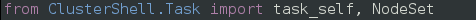
\includegraphics[scale=0.7]{from_clustershell.png}
\caption{Import}
\end{figure}

\pagebreak
\section{Script gestion des services}
\label{sec:section3}
\subsection{Présentation}
\label{sub:3.1}

Cette première partie consiste créer un script en python permettant d'utiliser les fonctionnalités de base des services, en étendant cette fonctionnalité de façon distribuée sur un ensemble choisi de noeuds.
Pour ce faire, on utilise l'api python Clustershell qui va nous permettre de créer un script pouvant effectuer ces actions.


\pagebreak


\section{Script avec fichier de configuration}
\label{sec:section4}
\pagebreak

\section{Création d'une IHM}
\label{sec:section5}
Pour la création d'une interface graphique, nous nous sommes tournés vers l'environnement de développement Qt. Qt est basé sur le langage C++ pour créer ses IHM. Cependant il existe le module PyQt permettant de programmer en python une interface graphique aisément.
\subsection{Qt Creator et PyQt}
\subsubsection{La conversion ui > py}
Au départ, on utilise Qt Creator pour pouvoir créer les fenêtres avec tous les composants nécessaires. Lorsque l'on créé une fenêtre, Qt nous génère un fichier \textbf{.ui}. A l'aide de l'utilitaire \textbf{pyuic}, on peut convertir ce fichier en python.
\begin{figure}[hbtp]
\centering
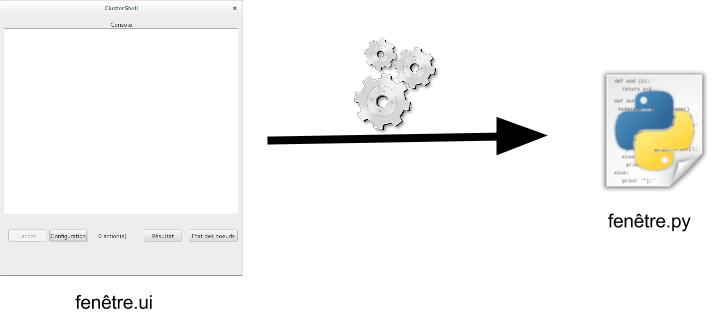
\includegraphics[scale=0.3]{conversion_ui_py.jpg}
\caption{Conversion ui - py}
\end{figure}
Pour convertir on utilise la commande suivante: \textbf{pyuic4 fenêtre.ui > fenêtre.py}\linebreak
\\
\subsubsection{Les classes d'interfaces graphique}
Dans notre fichier python (qui représente la fênetre) se trouve au final une classe qui porte le nom \textbf{Ui\_Form} pour une fenêtre ou \textbf{Ui\_MainWindow} si c'est la fenêtre principale. Das cette classe se trouve une fonction qui s'appelle \textbf{setupUI} et qui configurer tous les composants graphiques qui se trouve dans la fenêtre (exemple: un bouton avec sa taille de base, sa taille maximum etc...). C'est la première fonction à être appelé lors du lancement de la fenêtre.
\linebreak
Voici comment se déroule l'initialisation d'une fenêtre
\begin{center}
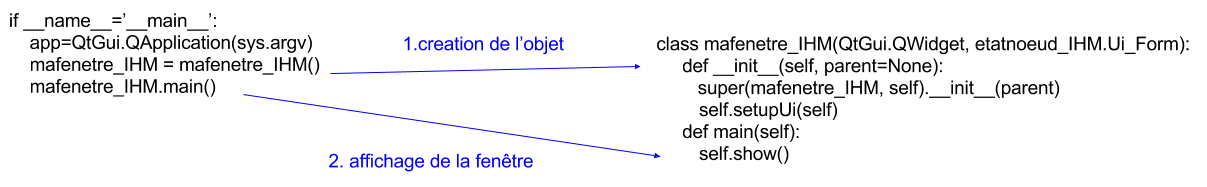
\includegraphics[scale=0.45]{initialisation_fenetre.jpg} 
\end{center}


\subsubsection{Les signaux et les slots}
Pour de la programmation événementielle, on utilise deux moyens qui sont propres à Qt: les signaux et les slots. Chaque composant graphique (comme un bouton) possède des signaux et des slots qui vont permettre d'intéragir avec d'autres composants et fonctions(exemple: ouvrir une fenête via un bouton).\\
\linebreak
\textbf{Un signal:} Un signal est un message envoyé par une classe lors du déclenchement d'un événement comme le clic sur un bouton\\
\textbf{Les slots:} Les slots sont tout simplement des fonctions qui seront déclenchés par les signaux. Les fonctions peuvent être créés par nous même ou cela peut être des fonctions propres à une classe de Qt( exemple: la fonction \textbf{quit} de \textbf{QApplication} qui quitte le programme.\\
Voici un petit exemple pour mieux comprendre:\\
\begin{figure}[hbtp]
\centering
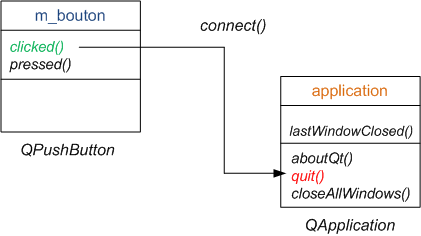
\includegraphics[scale=0.5]{exemple_signal_slot.png}
\caption{Les signaux et slots}
\end{figure}\\
Pour pouvoir assigner un slot à un signal on doit utilise la fonction \textbf{connect} que l'on définit dans la classe de notre fenêtre:
\begin{center}
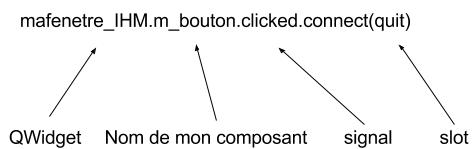
\includegraphics[scale=0.4]{signal_slot.jpg} 
\end{center}
La définiton d'un slot ce fait exactement de la même manière que celle d'une fonction de base. Il faut également ajouter "\textbf{@pyqtSlot()}" devant la fonction. C'est grâce à pyqtSlot que Qt va savoir que ce sont des slots et non des fonctions.\\
Voici un exemple de slot:
\begin{lstlisting}
@pyqtSlot()
def monslot():
   print "Hello World"
\end{lstlisting}

\subsubsection{Le programme principal}

Comme dans tout fichier python, une fonction main existe et doit être appelé pour lancer le programme principal. Le fichier python principal (\textbf{IHM.py}) va contenir:
\begin{itemize}
\item Les signaux et les slots
\item Les classes d'interface graphique
\item Le code lié aux interactions avec les composants graphiques
\end{itemize}
\subsubsection{Arborescence des fichiers}
Afin de mieux comprendre comment notre IHM à été créé, voici un récapitulatif de l'ensemble de nos fichiers python est regroupé dans le dosser clustershell\_IHM.\\
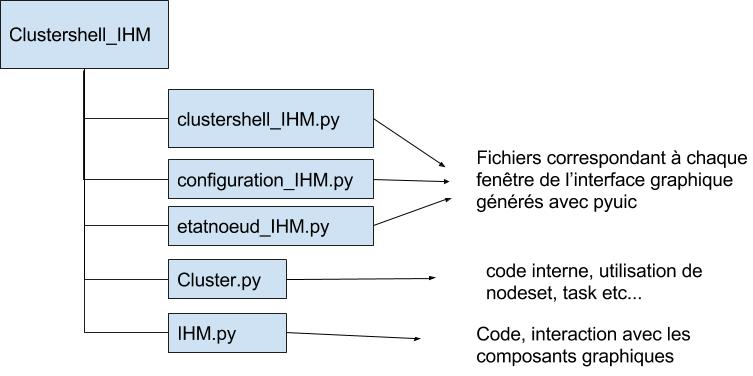
\includegraphics[scale=0.5]{arborescence_fichiers_IHM.jpg} 

\subsection{Visualisation des résultats}
\begin{center}
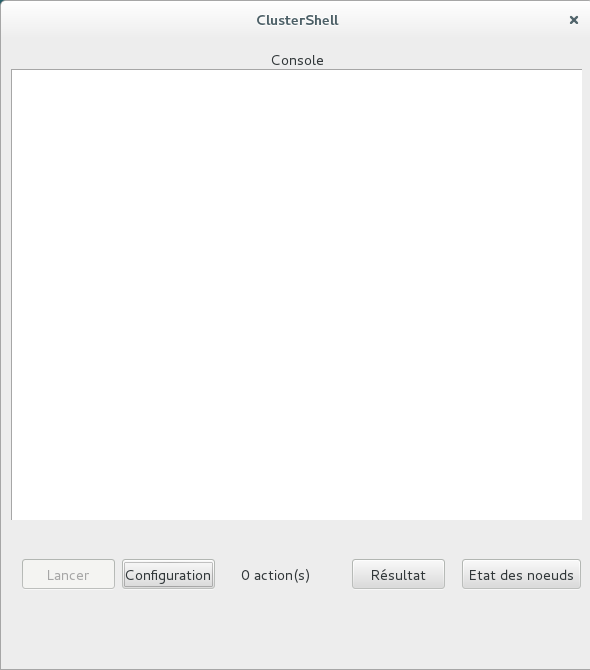
\includegraphics[scale=0.6]{fenetre_principale.png} 
\end{center}
La fenêtre principale est le point d'entrée de notre IHM, elle va permettre de visualiser la sortie de chaque noeud de notre cluster et d'analyser rapidement les résultats.\\
Tout d'abord nous avons mis en place une autre fenêtre (accessible via le bouton "Etat des noeuds") permettant de vérifier l'état de noeuds. Ensuite nous pouvons configurer nos noeuds (via la fenêtre de configuration accessible via le bouton "Configuration").\\
De plus nous avons trouvé qu'il était essentiel de garder une trace des résultats de tous les noeuds alors vous avons gardé en mémoire ces résultats dans des fichiers qui sont crées à partir du bouton "Résultat".

\subsection{Configuration des services}

\subsection{Vérification de l'état des noeuds}

\begin{center}
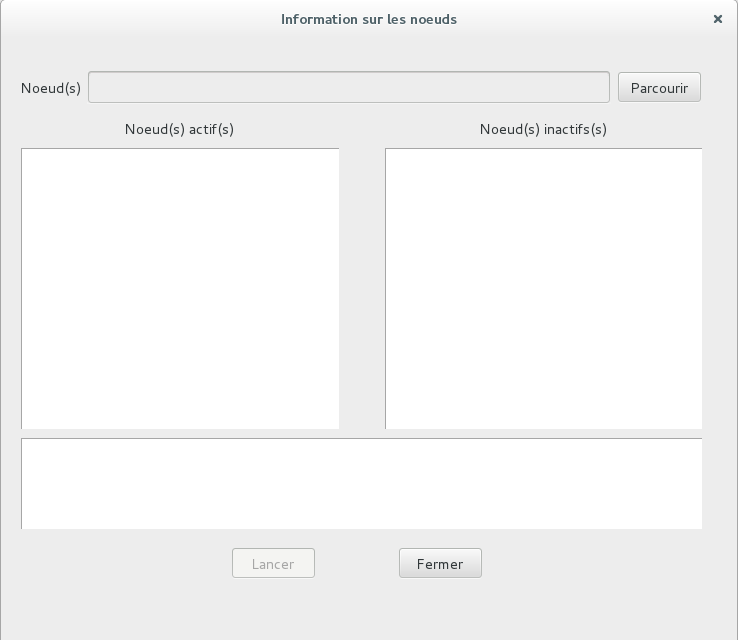
\includegraphics[scale=0.6]{fen_etat_noeud.png} 
\end{center}

Il est souvent utile de savoir si un noeud est bien présent ou non pour effectuer une quelconque tâche. On a alors créé une fenêtre permettant de lister les noeuds actifs et les noeuds qui ne répondaient.\\
On a utilisé en tout 3 \textbf{QListWidgets}; une pour les noeuds actifs, une pour les noeuds qui ne répondaient pas et une dernière pour l'affichage des erreurs.\\
Si l'utilisateur veut tester ses noeuds, il dispose de deux choix:
\begin{itemize}
 \item Chercher le(s) noeud(s) qu'il veut vérifier en les renseignant dans la barre de saisie (\textbf{QLineEdit} )
 \item Si jamais l'utilisateur avait déjà écris sont fichier au format YAML pour pouvoir administrer ses services, il peut à par avance tester les noeuds dans ce noeud. Le fichier est récupérer via le bouton (\textbf{QPushButton}) "Parcourir".
 \end{itemize}
\subsubsection{Test des noeuds via la barre de saisie}
Lorsque l'utilisateur tape une liste de noeuds et lance la vérification des noeuds via le bouton "Lancer", on utilise un signal qui va appeler une fonction de vérification des noeuds:\\
\begin{lstlisting}
etatnoeud_IHM.pushButton.clicked.connect(check_etat_noeud)
\end{lstlisting}
\textbf{Partie de la fonction de vérification des noeuds:}\\
Pour tester si les noeuds sont actifs on a finalement lancé une commande sur le(s) noeud(s) en question et on à vérifié si le résultat était bien celui qu'on attendait. Ici j'ai simplement utilisé la commande "\textbf{echo Hello}".\\
Voici le code qui vérifie la présence et gère l'affichage des noeuds sur l'interface graphique:
\begin{flushleft}
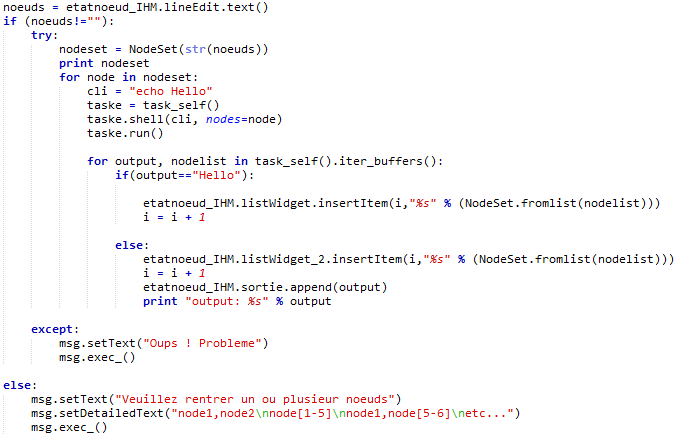
\includegraphics[scale=1]{check_etatnoeud.png} 
\end{flushleft}
Détail du code:\\
\begin{enumerate}
\item Utilisation de \textbf{NodeSet} pour vérifier si ce que l'utilisateur a tapé correspond à la syntaxe d'un noeud.
\item Utilisation de \textbf{Task} pour lancer la commande sur le(s) noeud(s)
\item La boucle for permet de récupérer le résultat d'exécution de la commande sur les noeuds.
\begin{itemize}
\item Si la sortie (\textbf{output}) correspond bien à "Hello", on récupère le nonom du noeud et on l'ajoute dans la \textbf{QListWidget}.
\item Sinon on l'ajoute dans l'autre \textbf{QListWidget} qui liste les noeuds non actifs.
\end{itemize}
\item Biensur on vérifie si quelque chose à bien été entré dans la barre de saisie. L'objet \textbf{msg} de type \textbf{QMessageBox} va afficher une boite de dialogue:\\
\linebreak
\begin{center}
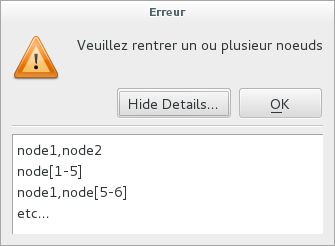
\includegraphics[scale=0.8]{messagebox.png} 
\end{center}

\end{enumerate}
 




\subsubsection{Test des noeuds via un fichier}
Lors de l'ouverture du fichier au format YAML, il était nécessaire de tester avant tout si la syntaxe du fichier était correcte. Cependant cette vérification à déjà été faite auparavant lors de l'importation d'un fichier au niveau de la configuration des services.\\
Comme les fonctions utilisés n'etaient pas entièrement compatible avec le contexte il a fallu écrire de nouvelles fonctions basé sur les anciennes en les modifiant.\\
\begin{figure}[hbtp]
\centering
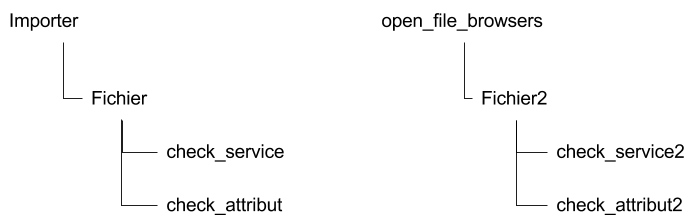
\includegraphics[scale=0.5]{difference_importer_openfile.png}
\caption{Fonctions de configuration vs Fonctions de vérification de noeuds}
\end{figure}

\subsection{Configuration des noeuds}

\subsection{Mise en place des résultats d'exécution dans des logs}
\section{Sources}
\label{sec:section6}
\subsection{Références}
\textbf{Nodeset:} \url{http://clustershell.readthedocs.io/en/latest/api/NodeSet.html}\\
\textbf{Task:} \url{http://clustershell.readthedocs.io/en/latest/api/Task.html}\\
\textbf{Qt GUI:} \url {http://doc.qt.io/qt-4.8/qtgui-module.html}\\
\url {https://pythonspot.com/en/pyqt4/}\\
\url {http://pyqt.sourceforge.net/Docs/PyQt4/qtgui.html} 

\end{document}